% Created 2023-01-31 Tue 16:46
% Intended LaTeX compiler: xelatex
\documentclass[11pt,twoside,landscape]{article}
\usepackage{graphicx}
\usepackage{longtable}
\usepackage{wrapfig}
\usepackage{rotating}
\usepackage[normalem]{ulem}
\usepackage{amsmath}
\usepackage{amssymb}
\usepackage{capt-of}
\usepackage{hyperref}
\usepackage{subcaption}
\usepackage[newfloat]{minted}
\usepackage{color}
\usepackage{listings}
\usepackage[top=2cm,bottom=2cm,right=2cm,left=2cm,landscape]{geometry}
\usepackage{multicol}
\usepackage{enumitem}
\usepackage{fancyhdr}
\usepackage{caption}
\usepackage{algorithm}
\usepackage{algpseudocode}
\usepackage{float}
\setlist{noitemsep}
\setlength{\parindent}{0pt}
\setlength{\columnseprule}{0.2pt}
\definecolor{mygreen}{rgb}{0,0.6,0}
\definecolor{mygray}{rgb}{0.5,0.5,0.5}
\definecolor{mymauve}{rgb}{0.58,0,0.82}
\lstset{ backgroundcolor=\color{white}, basicstyle=\footnotesize, breaklines=true, captionpos=b, commentstyle=\color{mygreen}, escapeinside={\%*}{*)},keywordstyle=\color{blue}, stringstyle=\color{mymauve},}
\author{Olivier Lischer}
\date{\today}
\title{PF Summary}
\hypersetup{
 pdfauthor={Olivier Lischer},
 pdftitle={PF Summary},
 pdfkeywords={},
 pdfsubject={},
 pdfcreator={Emacs 27.2 (Org mode 9.5.5)}, 
 pdflang={English}}
\begin{document}

\pagestyle{fancy}
\fancyhf{}
\fancyhead[R]{PF-HS22}
\fancyhead[L]{Summary}
\fancyfoot[CE,CO]{\leftmark}
\fancyfoot[R]{\thepage}
\fancyfoot[L]{Olivier Lischer}

\tableofcontents
\newpage

\begin{multicols}{3}
\section{Patterns}
\label{sec:orgb03538d}
\subparagraph{What is a Pattern} \
\label{sec:orga345d4e}
The GoF had 4 elements for specifying a design pattern.
Today you have 6:
\begin{description}
\item[{Context}] What is your task, give a little background information
\item[{Intent}] What do you want to solve?
\item[{Forces}] What does it make hard to solve this problem?
\item[{Benefits}] What is positive when implemented?
\item[{Liabilities}] What does it cost you?
\end{description}


Example:
\begin{itemize}
\item Context: Design a waiting room
\item Intent: efficient use of time
\item Forces: different needs of different people
\item Benefits: well-being \(\uparrow\)
\item Liabilities: Costs
\end{itemize}
\subparagraph{Pattern Language} \
\label{sec:orgd647590}
A Pattern Languages combine patterns according to their relationships.
If you have established a Pattern Language, you can read a text and just insert the name of the patterns, and it does make sense.
\section{GoF}
\label{sec:org1acd697}
\subparagraph{Mediator} \
\label{sec:org92dd46b}
The Mediator Design Pattern is used to encapsulate how a set of objects interact with each other.
The different objects do not have to reference each other explicit.

{
\begin{center}
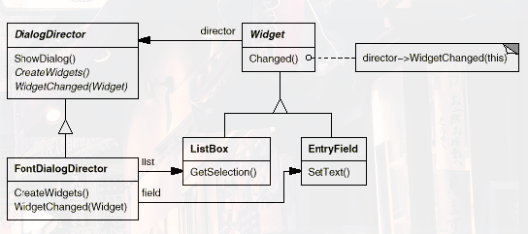
\includegraphics[width=.9\linewidth]{img/mediator.png}
\end{center}
\captionof{figure}{Mediator Class Diagram}\label{fig:mediator-class-diagram}
}

\begin{enumerate}
\item How does it work?
\label{sec:org53740e4}
The mediator holds a reference to every object.
The user selected some item from the list box (object A).
Object A notifies the mediator that the value has changed.
The mediator know notifies the other objects.

{
\begin{center}
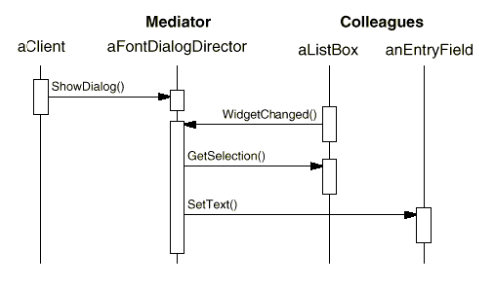
\includegraphics[width=.9\linewidth]{img/mediator_sequence_diagram.png}
\end{center}
\captionof{figure}{Mediator Sequence Diagram}\label{fig:mediator-sequence-diagram}
}
\end{enumerate}

\subparagraph{Memento} \
\label{sec:org06b5bcc}
The Memento Design Pattern is used to store an internal state.
This is often used for restoring the internal state of an object.

The object creates a memento (a copy of the state itself) and returns it to the world.
The state of the object can be restored using such a memento.
You can not change the memento and the inner live is unknown to the outer world.


{
\begin{center}
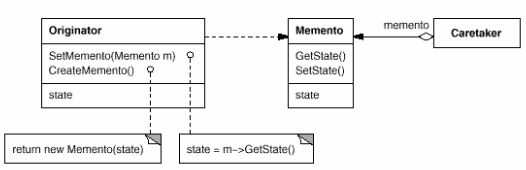
\includegraphics[width=.9\linewidth]{img/memento.png}
\end{center}
\captionof{figure}{Memento Class Diagram}\label{fig:memento-class-diagram}
}
\subparagraph{Command} \
\label{sec:org0c514e5}
The command pattern is used to encapsulate actions / request inside an object.
For example, the design of a framework does not know which action the button should perform.
Therefore, the button is created using a command as parameter.
As soon as the user clicks on the button, the button executions the \texttt{command.Execute()} function.

{
\begin{center}
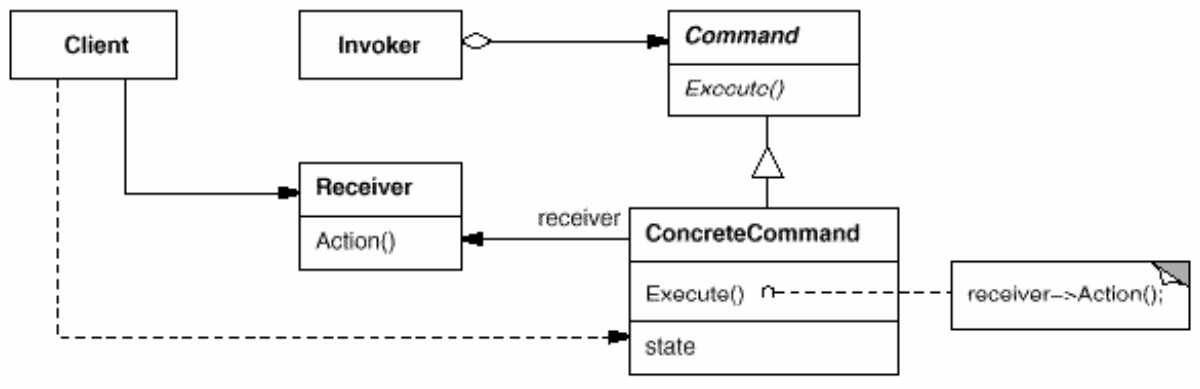
\includegraphics[width=.9\linewidth]{img/command.png}
\end{center}
\captionof{figure}{Command Class Diagram}\label{fig:command-class-diagram}
}

{
\begin{center}
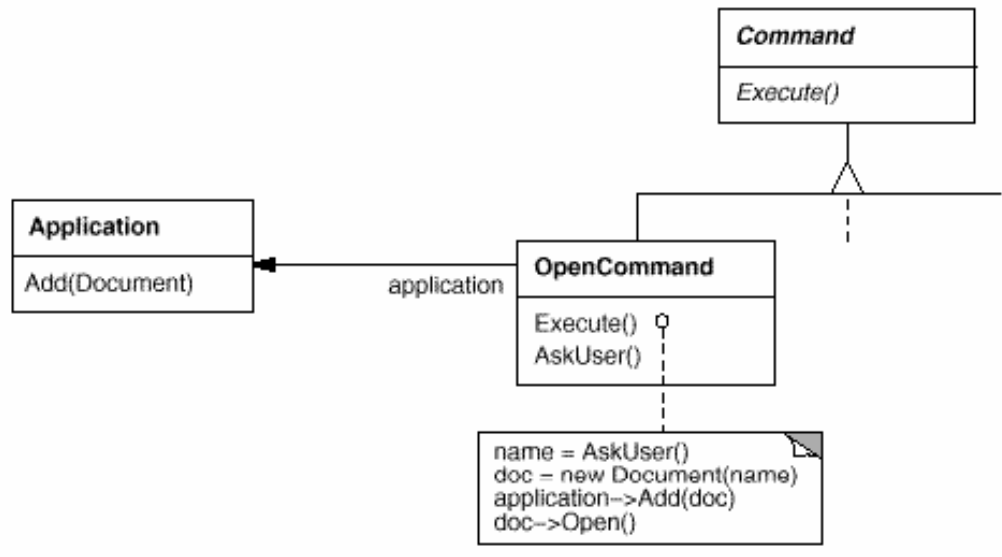
\includegraphics[width=.9\linewidth]{img/example_of_command.png}
\end{center}
\captionof{figure}{Example of Command Pattern}\label{fig:example-of-command-pattern}
}
\subparagraph{Command Processor} \
\label{sec:org297fabd}
The Command Processor is an extension of the Command Pattern.
The Command Processor is more or less just a \href{../../../roam/20210806220134-stack.org}{Stack} of Commands.

The Command Processor gets the command (\texttt{do\_it}).
If you want to undo more than one command you just call \texttt{undo\_it} multiple times on the processor.


{
\begin{center}
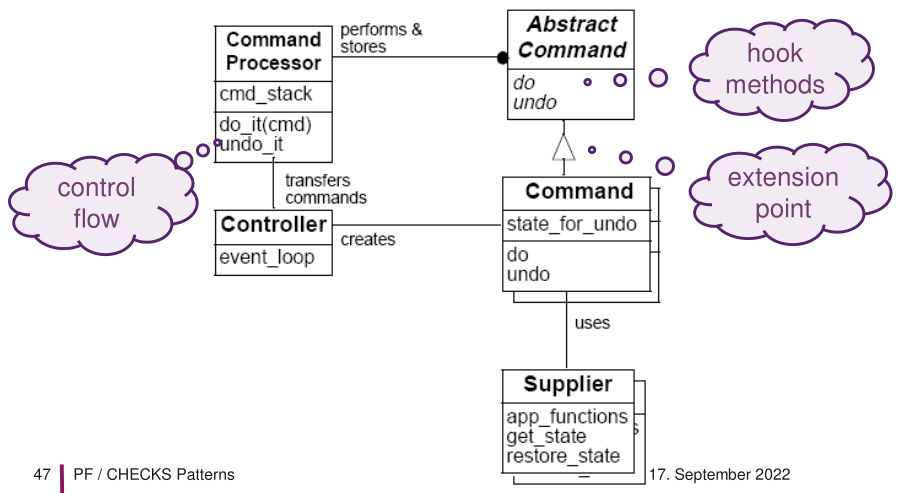
\includegraphics[width=.9\linewidth]{img/command_processor.png}
\end{center}
\captionof{figure}{Command Processor}\label{fig:command-processor}
}
\subparagraph{Visitor} \
\label{sec:org06eda8d}
The Visitor Patter is used to "visit" class hierarchy.
The visitor can perform action on the visited elements (for example spell checking in a document).

It is easy to implement a new Visitor (Just implement the Interface).
However, extending the class hierarchy with a new subclass is very difficult.
You have to extend the interface \texttt{Visitor} and therefore all implementations of this interface.

{
\begin{center}
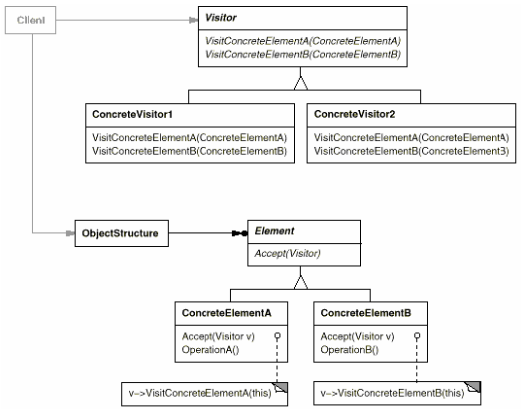
\includegraphics[width=.9\linewidth]{img/visitor.png}
\end{center}
\captionof{figure}{Visitor Class Diagram}\label{fig:visitor-class-diagram}
}

{
\begin{center}
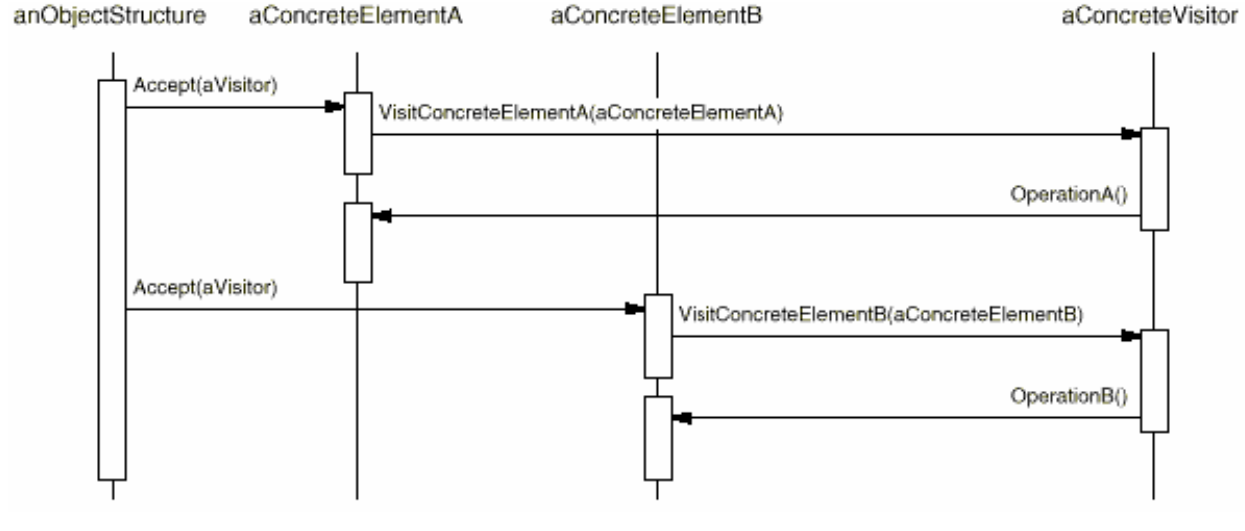
\includegraphics[width=.9\linewidth]{img/visitor_sequence.png}
\end{center}
\captionof{figure}{Visitor Sequence}\label{fig:visitor-sequence}
}

\subparagraph{(External) Iterator} \
\label{sec:org2073614}
The iterator design pattern is used to access the items in a \href{../../../roam/20210518131131-datastructure.org}{Data structure} (Aggregate in figure \ref{fig:iterator-class-diagram}).
The benefit of iterator is that it hides the implementation details of the data structure.

\begin{lstlisting}[language=rust,label= ,caption= ,captionpos=b,numbers=none]
let my_vec = vec![1, 10];
let iter = my_vec.iter();
let _ = iter.next();
let _ = iter.next();
// ...
\end{lstlisting}


{
\begin{center}
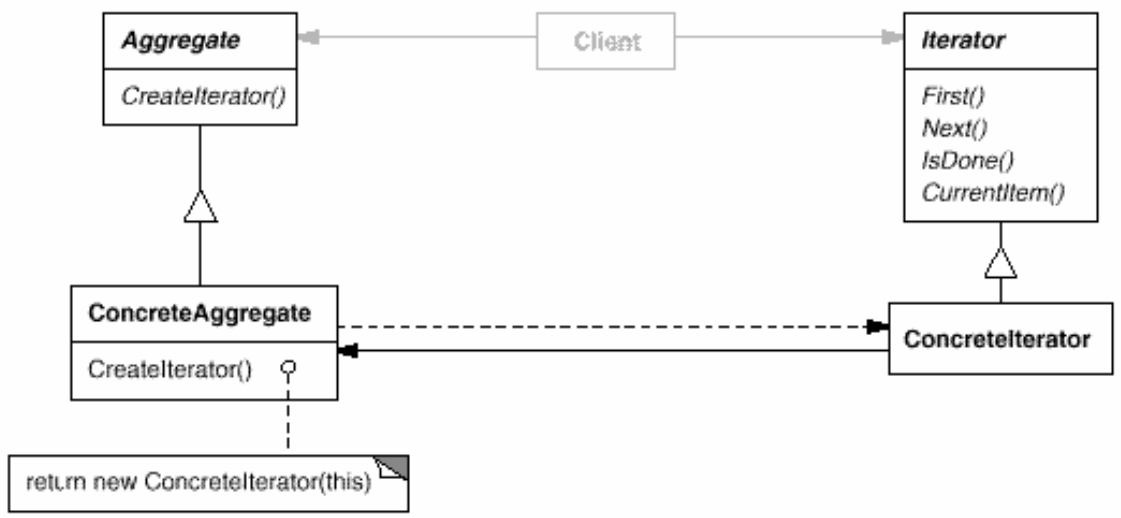
\includegraphics[width=.9\linewidth]{img/iterator.png}
\end{center}
\captionof{figure}{Iterator Class Diagram}\label{fig:iterator-class-diagram}
}
\subparagraph{Internal Iterator} \
\label{sec:orgd6b1c35}
The internal Iterator is used to iterate over a data structure.
In contrast to the \href{../../../roam/20220413201100-design_pattern_iterator.org}{Design Pattern - External Iterator} you provide a function, which is called for each element.

\begin{lstlisting}[language=csharp,label=lst:internal-iterator-examples,caption={Internal Iterator Examples},captionpos=b,numbers=none]
List<T>.ForEach(Action<T>); // C#
Collection.forEach(); // Java
Stream.forEach(); // Java
Array.prototype.forEach(); // JS
\end{lstlisting}
\subparagraph{State} \
\label{sec:orgc387691}
The state pattern is used allow an object to alter its internal behavior depending on its state.
The object will appear to change its class.

\begin{center}
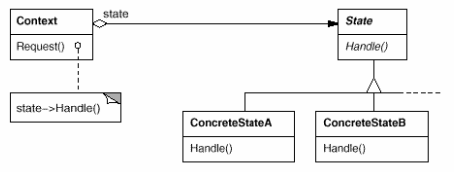
\includegraphics[width=.9\linewidth]{img/state.png}
\end{center}
\captionof{figure}{State Class Diagram}\label{fig:state-class-diagram}
\begin{center}
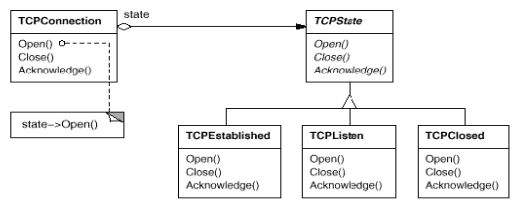
\includegraphics[width=.9\linewidth]{img/state_example.png}
\end{center}
\captionof{figure}{TCP Connection with State}\label{fig:tcp-connection-with-state}

\subparagraph{Method for States} \
\label{sec:org975d21e}
The Methods for States Pattern is a derivation of the State Pattern by GoF.
A State is represented as a collection of functions (struct, HashMap, enum, \ldots{}).
The State Machine itself stores such a collection of function inside and just executes the function on the struct.


{
\begin{center}
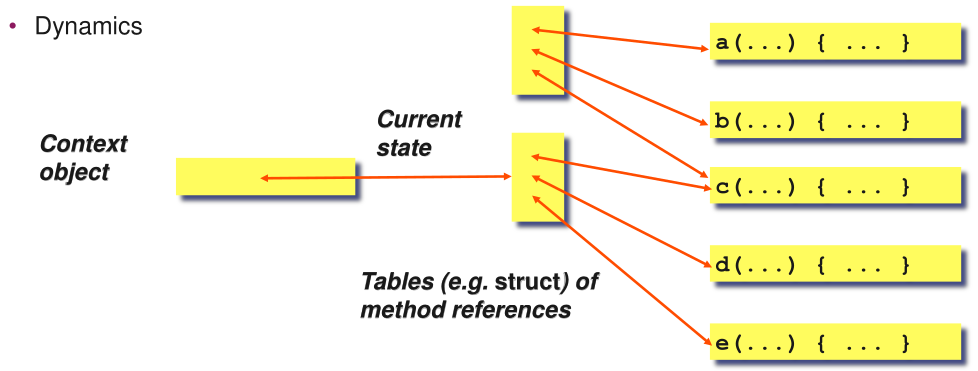
\includegraphics[width=.9\linewidth]{img/methods_for_states.png}
\end{center}
\captionof{figure}{Methods For State Example}\label{NAME: Methods For State Example}
}
\subparagraph{Collection for States} \
\label{sec:orgdbff90c}
Collection for States is a way to handle multiple objects in a particular state.
For each state you have a list / collection, which contains the objects in this state.

If an event is triggered, then the event is executed on all objects in the list, which should handle this.
The distinction between the states is made depending on which list / collection the work item is.
\subparagraph{Factory Method} \
\label{sec:org4ef9ee5}
The Factory Method is used to create an object, but the subclass decides which class is instantiated.
With this pattern you can create concrete creators which can decide which concrete product should be created.
The user of the creator only has to use the interface.


{
\begin{center}
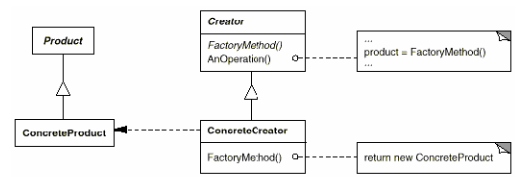
\includegraphics[width=.9\linewidth]{img/factory_method.png}
\end{center}
\captionof{figure}{Factory Method Class Diagram}\label{fig:factory-method-class-diagram}
}
\subparagraph{Template Method} \
\label{sec:org39161cf}
Using the Template Method Pattern you write the skeleton for an algorithm in the base class.
The functions which do something with data can be overwritten in a subclass.

{
\begin{center}
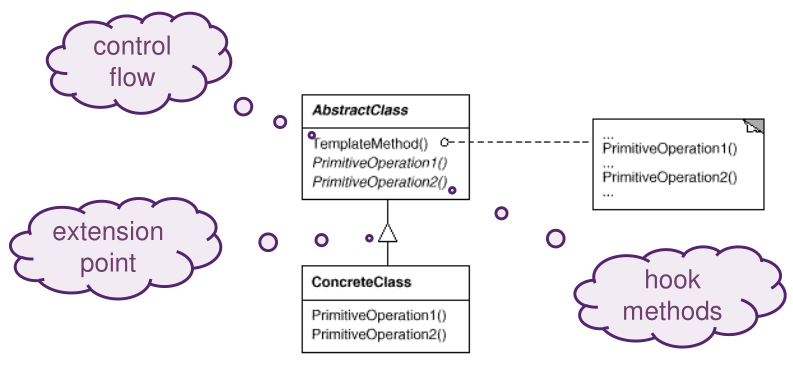
\includegraphics[width=.9\linewidth]{img/template_method.png}
\end{center}
\captionof{figure}{Template Method Class Diagram}\label{fig:template-method-class-diagram}
}
\begin{enumerate}
\item Example
\label{sec:org7b37bd9}
In an algorithm to traverse a tree in order you can implement a function \texttt{handleData()}.
This function is called every time when the element is "in order".
You have now one implementation of the algorithm, but you can handle the data differently using subclasses.
\end{enumerate}

\subparagraph{Strategy} \
\label{sec:orga9a2634}
The Strategy Pattern is used to encapsulate an algorithm in an object.
With this approach you can change the algorithm at runtime.

{
\begin{center}
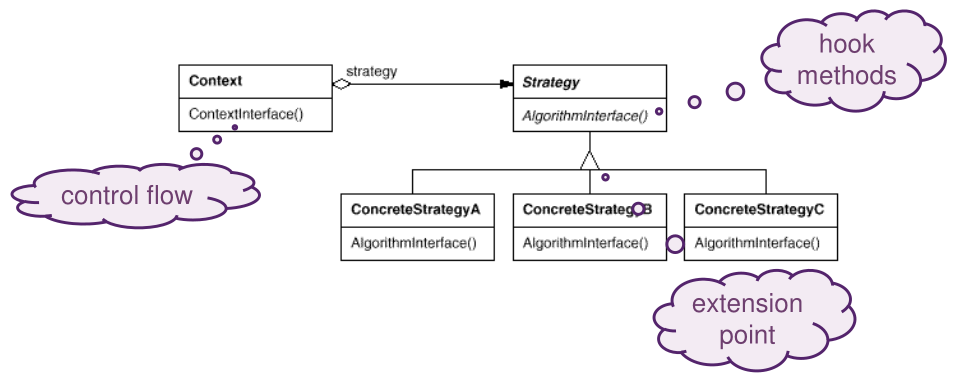
\includegraphics[width=.9\linewidth]{img/strategy_pattern.png}
\end{center}
\captionof{figure}{Strategy Class Diagram}\label{fig:strategy-class-diagram}
}
\subparagraph{Flyweight} \
\label{sec:orgefcf572}
The Flyweight pattern is used to support large number of objects efficiently.
For example, you can store every character in its own object.
In a document with 1000 characters you need more than 1000 objects.
The Flyweight pattern helps here.

In the Flyweight class is only state indecent stuff stored.
Therefore, the Flyweight is shareable.
Instead, creating every time a new object with the character "a" you always reference to the same object.


{
\begin{center}
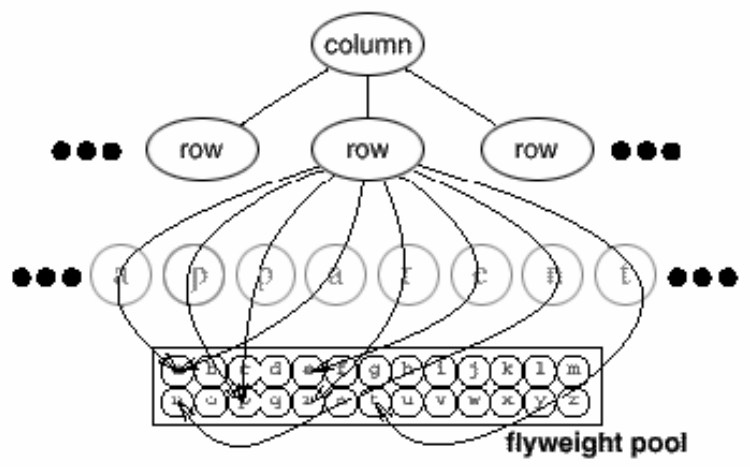
\includegraphics[width=.9\linewidth]{img/flyweight_example.png}
\end{center}
\captionof{figure}{Flyweight Example}\label{fig:flyweight-example}
}

{
\begin{center}
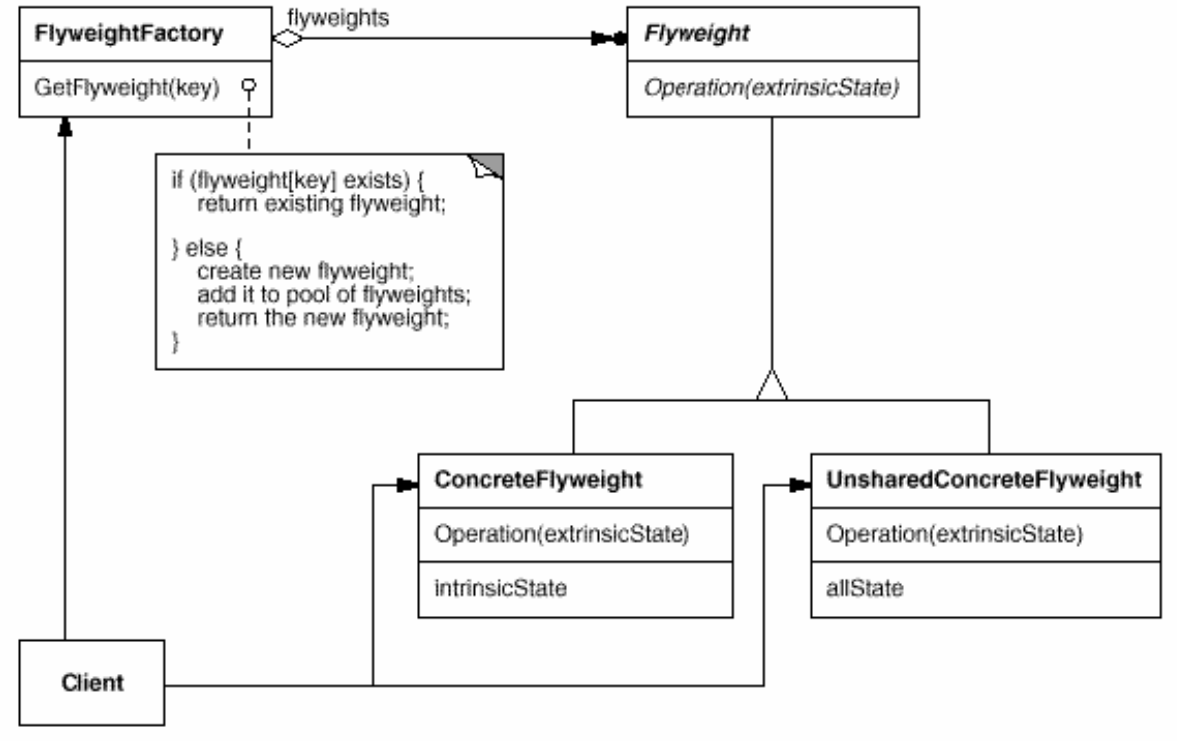
\includegraphics[width=.9\linewidth]{img/flyweight.png}
\end{center}
\captionof{figure}{Flyweight Class Diagram}\label{fig:flyweight-class-diagram}
}
\section{Value Patterns}
\label{sec:org622c666}
\subparagraph{Value Object} \
\label{sec:org9c950b5}
The Value Object Pattern is used to represent a class as values (immutable).
In \href{../../../roam/20201116150053-java.org}{Java} you don't have a Value Type \texttt{Year}.
Year however, is just a number.
With the Value Object Pattern you can simulate the same behavior for the Class \texttt{Year} as it was a type \texttt{int}.
The Identity is \textbf{not} important for such a type / value.


In \href{../../../roam/20211003114158-c.org}{C\#} just use the \texttt{struct} keyword.
In \href{../../../roam/20201116150053-java.org}{Java} use the \texttt{record} keyword.
However, you have to do some more stuff in Java.

\begin{quote}
«Override the methods in Object whose action should be related to content and not
identity and implement serializable.» [Henney]
\end{quote}

\begin{lstlisting}[language=java,label= ,caption= ,captionpos=b,numbers=none]
public final class Date implements Serializable {
    // …
    private static final long serialVersionUID = -3248069808529497555L;
    // …
    @Override
    public boolean equals(Object o) {
	if (this == o) return true;
	if (o == null || getClass() != o.getClass()) return false;
	Date date = (Date) o;
	return year.equals(date.year) && month.equals(date.month) && day.equals(date.day);
    }
    @Override
    public int hashCode() {
	return Objects.hash(year, month, day);
    }
}
\end{lstlisting}
\subparagraph{Whole Value} \
\label{sec:org3484a6d}
The Whole Value Pattern answers the following question:
\begin{quote}
How can you represent primitive quantities from your problem domain without loss
of meaning?

«Express the type of the quantity as a Value Class.» [Henney]
\end{quote}

The Whole Value can be immutable, but it is not required to be.

\begin{lstlisting}[language=java,label= ,caption= ,captionpos=b,numbers=none]
public final class Year {
    public Year(int year) { value = year; }
    public int getValue() { return value; }
    private final int value;
}

public final class Date {
    public Date(Year year, Month month, Day day) { /**/ }
    /**/
}
Date first = new Date(new Year(year), new Month(month), new Day(day));
\end{lstlisting}
\subparagraph{Enumeration Value} \
\label{sec:org6c7ecf3}
An enumeration value is just an Enum in \href{../../../roam/20201116150053-java.org}{Java}, \href{../../../roam/20211003114158-c.org}{C\#} or \href{../../../roam/20200904153952-rust.org}{Rust}.
\subparagraph{Immutable Value} \
\label{sec:orge4d029d}
An Immutable Value can not be changed.
That means all internal fields are \texttt{const} or \texttt{final}.

\begin{lstlisting}[language=csharp,label=lst:example-for-immutable-value,caption={Example for Immutable Value},captionpos=b,numbers=none]
struct Value {
    readonly int _value;
}
\end{lstlisting}
\subparagraph{Simple Factory} \
\label{sec:orgc3304af}
Intent:
\begin{itemize}
\item Provide an interface for creating objects without specifying the concrete implementation.
\end{itemize}

Motivation:
\begin{itemize}
\item You want to create concrete objects without knowing which concrete type you get.
\item You are only interested in the interface.
\end{itemize}
\subparagraph{Mutable Companion} \
\label{sec:org23ae38d}
\begin{quote}
How can you simplify complex construction of an Immutable Value?
\end{quote}


A Mutable Companion is a factory object for immutable values.
\texttt{StringBuilder} is an example for such a Mutable Companion for \texttt{Strings}.
For the final creation of the object (see \autoref{lst:example-for-mutable-companion}) you use the \href{../../../roam/20220413195351-design_pattern_factory_method.org}{Design Pattern - Factory Method}.

\begin{lstlisting}[language=java,label=lst:example-for-mutable-companion,caption={Example for Mutable Companion},captionpos=b,numbers=none]
var yearBuilder = new YearCompanion(Year.of(2020));
yearBuilder.next();
var nextYear = yearBuilder.asValue();

public final class YearCompanion {
    private int value;

    public YearCompanion(Year toModify) {
	this.value = toModify.getValue();
    }
    public void next() {
	this.value++;
    }
    public Year asValue() { // factory method
	return Year.of(value);
    }
}
\end{lstlisting}
\section{CHECKS Patterns}
\label{sec:orge7ff1d9}
\subparagraph{Exceptional Behavior} \
\label{sec:org67ab758}
\begin{quote}
How can exceptional behavior caused by invalid input be handled without throwing errors?
\end{quote}

If your function should indicate an error, but should not throw an error / exception then return an \emph{exceptional value} in an error case.
An \emph{exceptional value} could be:
\begin{itemize}
\item \texttt{null} or \texttt{undefined} (not recommended)
\item Enumeration Value to identify what went wrong
\end{itemize}


\begin{lstlisting}[language=js,label=lst:example-for-exceptional-behavior,caption={Example for Exceptional Behavior},captionpos=b,numbers=none]
export enum CalculationError {
    DivByZero = "div/0",
    NumeratorIsNaN = "NaN(numerator)",
    DivisorIsNaN = "NaN(divisor)"
}

export class Calculator {
    public static divide(numerator: number, divisor: number): number | CalculationError {
	if (divisor === 0) {return CalculationError.DivByZero; }
	if (isNaN(numerator)) {return CalculationError.NumertorIsNaN; }
	if (isNaN(divisor)) {return CalculationError.DivisorIsNaN; }

	return numerator / divisor;
    }
}
\end{lstlisting}
\subparagraph{Meaningless Behavior} \
\label{sec:orge63fe68}
\begin{quote}
Write methods (without) with minimalistic concern for possible failure.
\end{quote}

You will return a meaningless value unless a condition has domain meaning
\section{Framework}
\label{sec:org8eaa9fa}
\subparagraph{Framework} \
\label{sec:org3472158}
A framework is a collection of classes, functions, \ldots{} that are working together.
A framework provides \emph{hook} for \emph{extensions}.
In contrast to a library is, that the framework own the control flow and calls \textbf{your} components (\href{../../../roam/20230102153338-what_is_inversion_of_control.org}{Inversion of Control}).


Examples:
\begin{itemize}
\item Java
\begin{itemize}
\item Hibernate
\item Velocity
\end{itemize}
\item C\#
\begin{itemize}
\item .NET / Core
\item Entity Framework
\end{itemize}
\item JS
\begin{itemize}
\item Vue.js
\end{itemize}
\end{itemize}
\subparagraph{Application Framework} \
\label{sec:org64d09fe}
An Application Framework is a special kind of framework.
In a framework you use the framework, and you start the framework.
In an Application Framework the "main" method lives inside the application framework.

An example for an Application Framework is Eclipse.
Based on the Eclipse you can create many other products (Java IDE, C++ IDE, \ldots{}).

Examples:
\begin{itemize}
\item Java
\begin{itemize}
\item Spring (Boot)
\item Application Server (J2EE)
\end{itemize}
\item C\#
\begin{itemize}
\item ASP.NT
\end{itemize}
\item JS
\begin{itemize}
\item Angular
\end{itemize}
\end{itemize}
\section{Reflection}
\label{sec:orgb67cd5d}
\subparagraph{Reflection} \
\label{sec:org3438860}
Reflection consists of two aspects:
\begin{itemize}
\item \emph{Introspection} (observe own state, e.g. query object properties)
\item \emph{Intercession} (modify own state, e.g. add another attribute)
\end{itemize}

\begin{quote}
In computer science, reflective programming or reflection is the ability of a process to examine, introspect, and modify its own structure and behavior. [Wikipedia]
\end{quote}


\begin{lstlisting}[language=java,label= ,caption= ,captionpos=b,numbers=none]
if (origin instanceof Cloneable) {
    cloned = ((Cloneable)origin).clone();
} else {
    cloned = origin.getClass().getDeclaredConstructor().newInstance();
    // ...
    BeanUtils.copyProperties(origin, cloned); // get data from getters, fill into setters.
}
\end{lstlisting}
\subparagraph{Meta Level Programming} \
\label{sec:org8981247}
The \emph{Meta Level} provides a self-representaiton
\begin{itemize}
\item gives the software knowledge of its own structure
\item consists of \href{../../../roam/20230115160536-what_are_meta_objects.org}{Meta Objects}
\item interface for manipulation meta objects is called \href{../../../roam/20230115160651-what_is_the_metaobject_protocol.org}{Metaobject Protocol}
\end{itemize}


The \emph{base level} defines the application logic.

{
\begin{center}
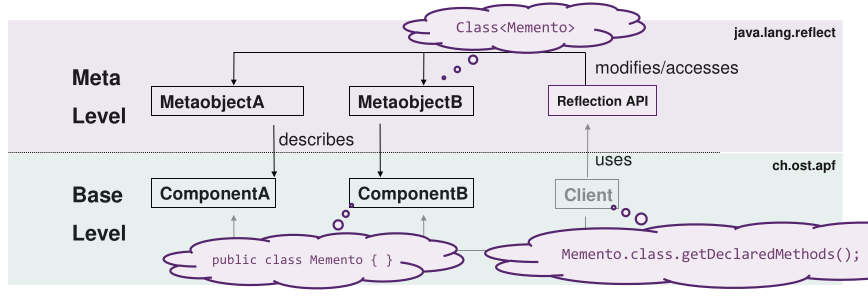
\includegraphics[width=.9\linewidth]{img/meta_base_level.png}
\end{center}
\captionof{figure}{Meta Level and Base Level}\label{fig:meta-level-and-base-level}
}
\subparagraph{Meta Object} \
\label{sec:orgcca959f}
If a programming language uses reflections it uses meta objects for:
\begin{itemize}
\item classes
\item object attributes
\item methods
\item class relationships
\item \ldots{}
\end{itemize}


{
\begin{center}
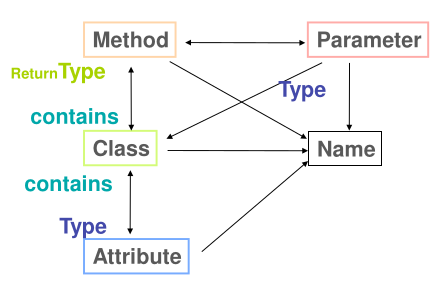
\includegraphics[width=.9\linewidth]{img/meta_object_relationships.png}
\end{center}
\captionof{figure}{Meta Object class relations}\label{fig:meta-object-class-relations}
}
\subparagraph{Meta Object Protocol} \
\label{sec:orgf0a56d4}
The Metaobject protocol provides a vocabulary to access and manipulate the structure and behavior of a system of objects.
\subparagraph{Pro / Con Reflection} \
\label{sec:org627e18d}
Benefits:
\begin{itemize}
\item Adapting a software system is easy
\item support for many kinds of changes
\end{itemize}


Liabilities:
\begin{itemize}
\item Produces non-transparent APIs
\begin{itemize}
\item control flow already hard to understand with polymorphism
\end{itemize}
\item binding at runtime (late binding)
\begin{itemize}
\item limited type safety (Rename class, but class name in string during reflection class is not renamed)
\item lower efficiency, no compiler-optimizaiton
\end{itemize}
\end{itemize}
\subparagraph{Type Object} \
\label{sec:orgc4b6b6f}
A Rental System contains books and videos.
For each book / video multiple copies may exist.
The descriptive information (title, author, actors) is stored in the book / video class (shared among copies).
Each media item type has own data and behavior.

{
\begin{center}
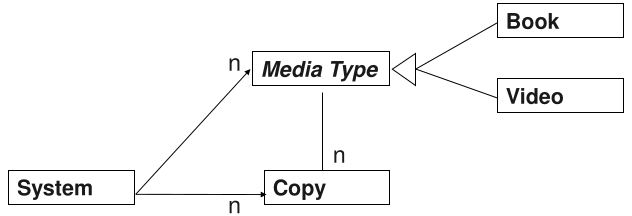
\includegraphics[width=.9\linewidth]{img/rental_system_example.png}
\end{center}
\captionof{figure}{Rental System Example}\label{fig:rental-system-example}
}
\textbf{Problem}:
\begin{itemize}
\item We want to keep common behavior and data in only one place
\begin{itemize}
\item object behavior depends on category (video / book)
\item categories should be objects themselves
\end{itemize}
\end{itemize}

\begin{quote}
How can you categorize objects, eventually dynamically?

Categorize objects by another object instead of a class (Book, Video)
Thus, an object can change 'class' at runtime.
\end{quote}


\textbf{Solution}:
\begin{itemize}
\item crate a category (\emph{type}) object which describes multiple objects
\item \emph{objects} forward the calls to the underlying type
\end{itemize}


{
\begin{center}
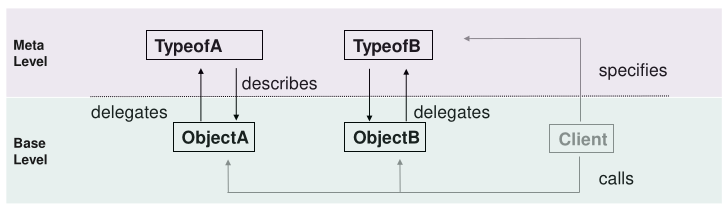
\includegraphics[width=.9\linewidth]{img/type_object_meta_base_level.png}
\end{center}
\captionof{figure}{Meta / Base Level Interactions}\label{fig:meta-base-level-interactions}
}

\begin{lstlisting}[language=java,label=lst:example-for-type-object,caption={Example for Type Object},captionpos=b,numbers=none]
// Base level
public class Copy {
    protected MediaType type;
    protected int copyid; // invoentory no

    public int getId() { return copyid; }
    // example for delegation
    public String getTypeid() { return type.getId(); }
    public String getTitle() { return type.getTitle() ;}
}

// Meta level
public class MediaType {
    protected String title;
    protected String typeid;

    public String getId() { return typeid; }
    public String getTitle() { return title; }
}
\end{lstlisting}
\subparagraph{Property List} \
\label{sec:org51a68ec}
\textbf{Problem}:
\begin{itemize}
\item attributes should be attachable / detachable after compilation
\item objects share attributes / parameters across the class hierarchy
\end{itemize}


\begin{quote}
How do you define properties (also arguments) in a flexible way, so they can be attached and detached at runtime?

Provide objects with a 'property list'. That list allows to associate names with other values or objects.
\end{quote}


\textbf{Solution}:
\begin{itemize}
\item property list maps attribute names to values
\item each name (e.g. a string) defines a slot / property
\end{itemize}

{
\begin{center}
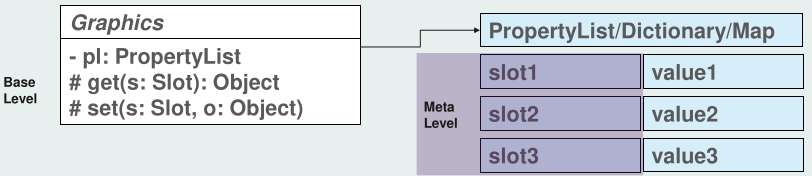
\includegraphics[width=.9\linewidth]{img/property_list_example.png}
\end{center}
\captionof{figure}{Property List Example}\label{fig:property-list-example}
}

\begin{lstlisting}[language=java,label=lst:example-for-anything,caption={Example for Anything},captionpos=b,numbers=none]
public class Graphics {
    private Properties pl;

    public String get(String prop) {
	return pl.getProperty(prop, "");
    }
    public void set(String prop, Object value) {
	pl.setProperty(prop, value);
    }
}

package java.util;
public class Properties {
    public Set<String> stringPropertyNames() { /**/ }
    public String getProperty(String prop, String defaultValue) { /**/ }
    public String setProperty(String prop, Object value) { /**/ }
}
\end{lstlisting}


\textbf{Benefits}:
\begin{itemize}
\item you can extend the object with properties at runtime while keeping object identity
\end{itemize}


\textbf{Liabilities}:
\begin{itemize}
\item Type safety left to the programmer (see \href{../../../roam/20230115180651-design_pattern_bridge_method.org}{Design Pattern - Bridge Method})
\item naming not checked by a compiler (see \href{../../../roam/20230115180651-design_pattern_bridge_method.org}{Design Pattern - Bridge Method})
\end{itemize}
\subparagraph{Anything} \
\label{sec:org7bf322d}
The Anything Pattern can be used to describe / create arbitrary data structure.
The Anything Pattern is something like a recursively structured Property List (\href{../../../roam/20230115171958-design_pattern_property_list.org}{Design Pattern - Property List})

An object is a collection of properties (property list) where you access the different values by name / key.
An array is a collection of properties (property list) where you access the different values by index.


{
\begin{center}
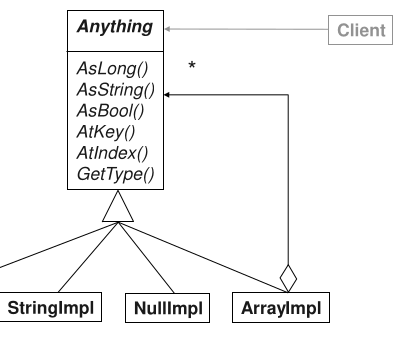
\includegraphics[width=.9\linewidth]{img/anything_pattern.png}
\end{center}
\captionof{figure}{Anything Class Diagram}\label{fig:anything-class-diagram}
}
\section{Singleton}
\label{sec:orgcbfcfca}
\subparagraph{Singleton} \
\label{sec:org9d165fe}
The Singleton pattern ensures that a class has only one (global) instance.
Additionally, it provides easy access to this element.

However, you should \textbf{NOT} use it in your software.
It is basically a global variable.
Therefore, not testable and difficult to maintain.

If you want something like singleton, you should use a simple factory which always returns the same instance.


\begin{lstlisting}[language=csharp,label=lst:singelton-alternative-in-code,caption={Singelton alternative in code},captionpos=b,numbers=none]
class SingletonFactory {
    private static object myInstance;

    createObject() {
	if (SingletonFactory.myInstance == null) {
	    SingletonFactory.myInstance = new();
	}
	return SingletonFactory.myInstance;
    }
}
\end{lstlisting}

{
\begin{center}
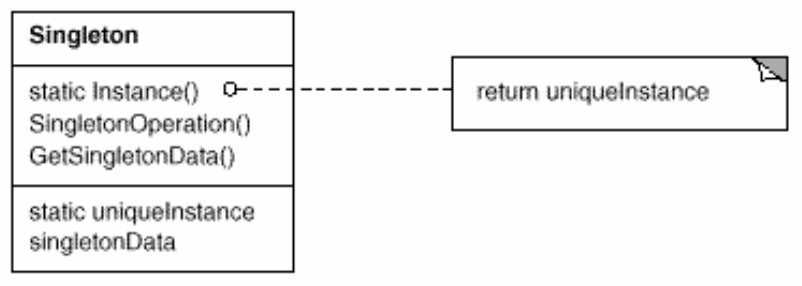
\includegraphics[width=.9\linewidth]{img/singleton.png}
\end{center}
\captionof{figure}{Singelton Class Diagram}\label{fig:singelton-class-diagram}
}
\subparagraph{Registry} \
\label{sec:orgeafc9db}
The Singleton Design Pattern is evil and should not be used.
An alternative could be the Registry pattern.

You will register multiple singletons in the registry.
Using a \texttt{lookup(name)} function you will get your specific singleton.
The \texttt{instance()} returns the default singleton from the registry.


{
\begin{center}
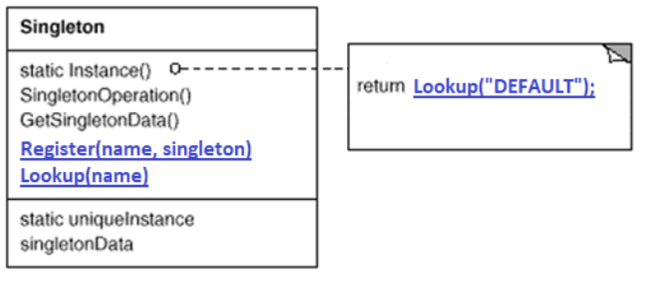
\includegraphics[width=.9\linewidth]{img/registry.png}
\end{center}
\captionof{figure}{Registry UML}\label{fig:registry uml}
}
\subparagraph{Monostate} \
\label{sec:org6e3a0a4}
If you have to use a framework, which provides a singleton you can kill this singleton using a \emph{Monostate}.
A monostate is a normal class, \textbf{but} all member variables are static members (see \autoref{lst:example-for-a-simple-monostate} and \autoref{lst:kill-a-singleton}).
\textbf{Attention:} In parallel and async execution you have to sync the access to static members.


\begin{lstlisting}[language=java,label=lst:example-for-a-simple-monostate,caption={Example for a simple monostate},captionpos=b,numbers=none]
public class Monostate {
    private static int x;
    private static int y;

    public int getX() { return x; }
    public int getY() { return y; }
}
\end{lstlisting}


\begin{lstlisting}[language=java,label=lst:kill-a-singleton,caption={Kill a singleton},captionpos=b,numbers=none]
public interface Monostate {
    int getX();
    int getY();
}

public class MonostateImpl implements Monostate {
    public int getX() {
	return Singleton.getInstance().getX();
    }

    public int getY() {
	return Singleton.getInstance().getY();
    }
}
\end{lstlisting}
\subparagraph{Service Locator} \
\label{sec:org59c8b33}
The Service Locator is a singleton, which only returns services or finders to find the concrete service.
The Service Locator is similar to a Registry.
If you use the Service Locator you have only \textbf{one} singleton in your application.

{
\begin{center}
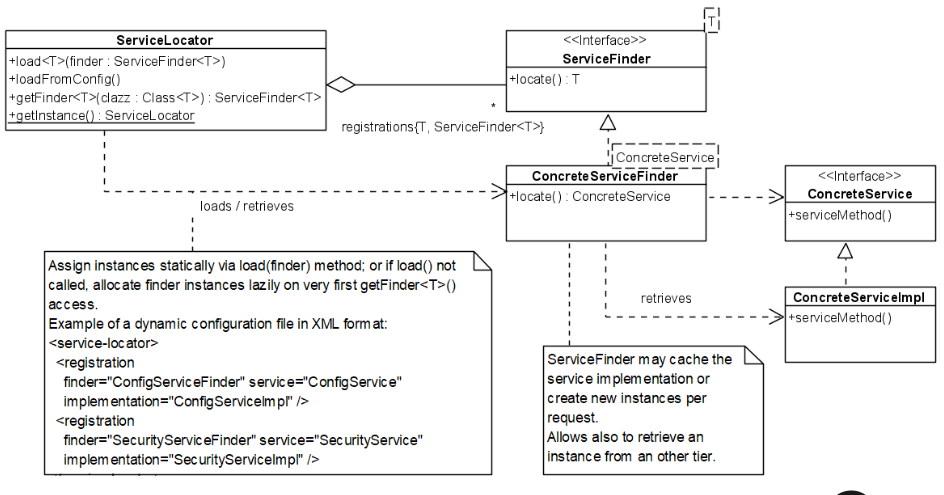
\includegraphics[width=.9\linewidth]{img/service_locator.png}
\end{center}
\captionof{figure}{Service Locator UML}\label{fig:service-locator-uml}
}

{
\begin{center}
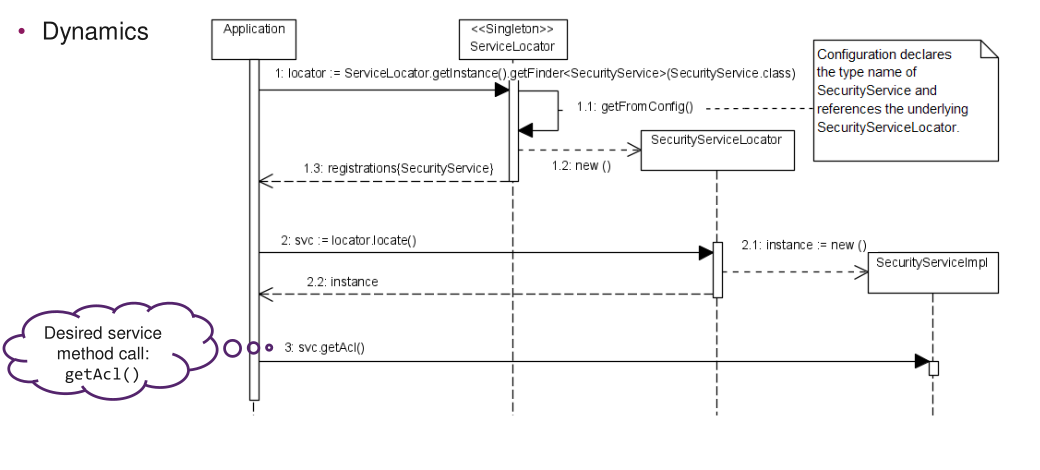
\includegraphics[width=.9\linewidth]{img/service_locator_dynamics.png}
\end{center}
\captionof{figure}{Service Locator Dynamics}\label{fig:service-locator-dynamics}
}

\subparagraph{Parameterize from Above} \
\label{sec:org6458356}
Often you have functionality which should be shared over multiple or all layers (configuration, security).
To solve this problem, without creating a singleton you can use \emph{Parameterize from Above}.
In the main method you will create all services.
And you provide all services over the constructor (form above, see \autoref{lst:example-for-parameteriz-from-above}).

{
\begin{center}
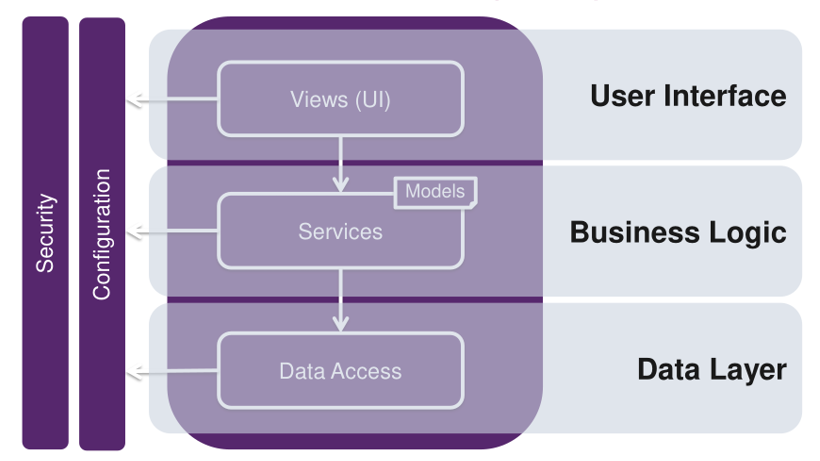
\includegraphics[width=.9\linewidth]{img/vertical_and_horizontal_layering.png}
\end{center}
\captionof{figure}{Horizontal and vertical layering}\label{fig:horizontal-and-vertical-layering}
}

\begin{lstlisting}[language=java,label=lst:example-for-parameteriz-from-above,caption={Example for Parameteriz from Above},captionpos=b,numbers=none]
public final class Bootstrapper {
    public static void main(string[] args) { // PfA applied
	// instantiate vertical layer contexts first
	SecurityContext securityContext = new SecurityContextImpl();
	ConfigurationSettings configuration = new ConfigurationSettingsImpl(args);
	// encapsulate variables into an application context
	var applicationContext = new ApplicationContextImpl(
							    securityContext,
							    configuration);
	// instantiate horizontal layer contexts from bottom to top
	DataContext dlContext = new DataContextImpl(applicationContext);
	BusinessContext blContext = new BusinessContextImpl(applicationContext, dlContext);
	UIContext uiContext = new UIContextImpl(applicationContext, blContext);
	// show initial UI dialog
	uiContext.show();
    }
}
\end{lstlisting}
\subparagraph{Dependency Injection} \
\label{sec:orge14ed24}
A Dependency Injection Container is used to store all services in a registry and injects the required services in the constructor while creating (\href{../../../roam/20230125163949-how_to_share_classes_over_multiple_layers.org}{Parameterize from Above}).

You register all services and components in the container.
The container will inject a compatible component according to your function signature.


{
\begin{center}
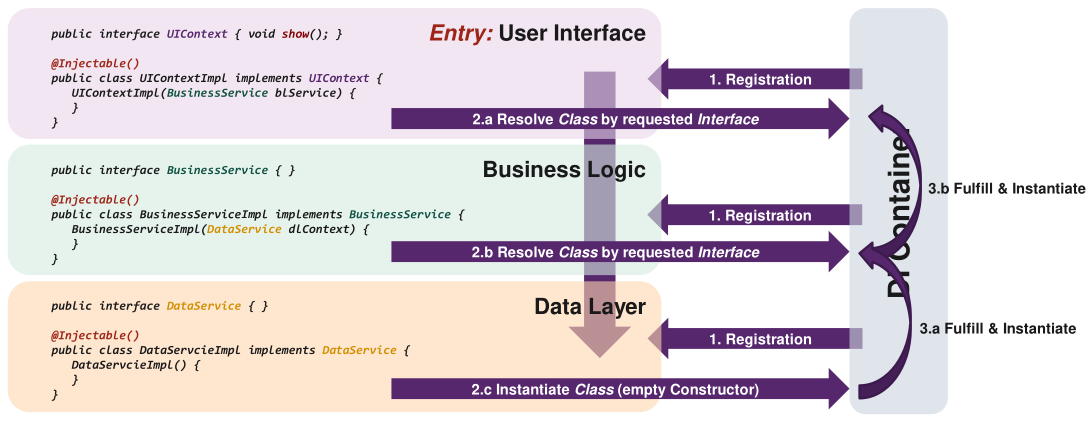
\includegraphics[width=.9\linewidth]{img/dependency_injection_example.png}
\end{center}
\captionof{figure}{Dependency Injection Example}\label{fig:dependency-injection-example}
}
\section{END}
\label{sec:org5ef54c8}
\end{multicols}
\end{document}